\input ../SlidePreamble
\input ../preamble

\begin{document}

{\Huge

  \centerline{\bf TTIC 31230, Fundamentals of Deep Learning}
  \bigskip
  \centerline{David McAllester, Winter 2019}
  \vfill
  \centerline{\bf Connectionist Temporal Classification (CTC)}
  \vfill
  \centerline{\bf and Deep Graphical Models}
\vfill
\vfill
\vfill

\slide{Distributions on Exponentially Large Sets}

\vfill
{\color{red}
$$\Phi^* = \argmin_\Phi E_{(x,y) \sim \mathrm{Pop}}\;-\ln \;P(y|x)$$

\vfill
$$\Phi^* = \argmin_\Phi E_{y \sim \mathrm{Pop}}\;-\ln \;P(y)$$
}

{\color{red} The structured case:} $y \in {\cal Y}$ where ${\cal Y}$ is discrete but {\color{red} iteration over $\hat{y} \in {\cal Y}$ is infeasible}.

\vfill
{\color{red} Language modeling} (unconditional) and {\color{red} machine translation} (conditional) are distributions on exponentially large (even infinite) sets.

\slide{Friendly and Unfriendly Distributions}

A model $P_\Phi(y)$ will be called {\color{red} friendly} if we can efficiently sample from it and, for any given $y$, can efficiently compute $P_\Phi(y)$.

\vfill
{\color{red} Autoregressive} language models (unconditional) and autoregressive machine translation models (conditional) are {\color{red} friendly}.


\vfill
Distributions which are not friendly in this sense will be called {\color{red} unfriendly}.

\slide{The Importance of Being Friendly}


{\color{red} If $P_\Phi(y|x)$ can be computed} (a friendly model)
we can do SGD on cross-entropy loss {\color{red} $- \ln P_\Phi(y|x)$} by back-propagating
through the computation of $P_\Phi(y|x)$.

\slide{Graphical Models}

\centerline{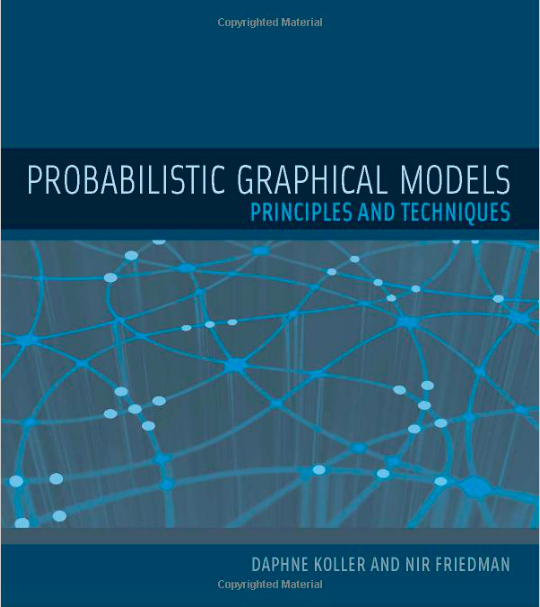
\includegraphics[height = 4in]{../images/Koller}}
\centerline{Koller and Friedman, MIT Press, 2009, 1270 pages}

\slide{Semantic Segmentation}
\centerline{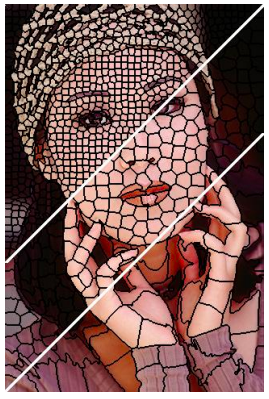
\includegraphics[height = 2.5in]{../images/SLICcolor}}
\centerline{\huge SLIC superpixels, Achanta et al.}

\vfill
We want to assign each superpixel one of $k$ semantic classes.

\vfill
For example ``person'', ``car'', ``building'', ``sky'' or ``other''.


\slide{General Markov Random Fields (MRFs)}

\centerline{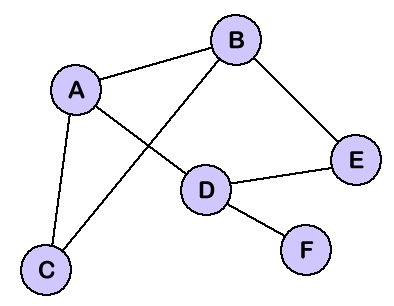
\includegraphics[height= 1.5in]{../images/Graph}}

$\hat{y} $ assigns a class $\hat{y}[i]$ to each node (superpixel) $i$.


$$s(\hat{y}) = \sum_{i \in \mathrm{Nodes}}\; s_i[\hat{y}[i]]\; + \sum_{e \in \mathrm{Edges}}\;s_e[\hat{y}[e.i],\hat{y}[e.j]]$$

\vfill
\centerline{Node Potentials \hspace{4em}Edge Potentials}

\slide{An Example}

Consider an image with three superpixels $A$, $B$ and $C$ where
each superpixel is to labeled as either ``foreground'' or background.

\vfill
Suppose the unary potentials are all zero.

\vfill
$$s_A(\mathrm{Foreground}) = s_A(\mathrm{Background}) = 0$$
$$s_B(\mathrm{Foreground}) = s_B(\mathrm{Background}) = 0$$
$$s_C(\mathrm{Foreground}) = s_C(\mathrm{Background}) = 0$$

\slide{The Binary Potentials}


\vfill
Let $F_A$ be the proposition that $A$ is forground and similarly for $F_B$ and $F_C$.

\vfill
We can express $F_A \Rightarrow F_B$ with
$$s_{A,B}(\mathrm{Foreground},\mathrm{Background}) = -1$$
$$s_{A,B}(\mathrm{Foreground},\mathrm{Foreground}) = 1$$
$$s_{A,B}(\mathrm{Background},\mathrm{Background}) = 1$$
$$s_{A,B}(\mathrm{Background},\mathrm{Foreground}) = 1$$

\vfill
The binary potentials are then given by
$F_A \Rightarrow F_B$, $F_B \Rightarrow F_C$, $F_C \Rightarrow F_A$.

\slide{The Full Configuration Potential}

For any configuration $\hat{y}$ we have that $s(\hat{y})$ is the sum of the unary and binary potentials.

\vfill
If none are foreground we have $s(\hat{y}) = 3$

\vfill
If one is foreground we have $s(\hat{y}) = -1 + 1+ 1 = 1$

\vfill
If two are foreground we also have $s(\hat{y}) = -1 + 1+ 1 = 1$

\vfill
If all are foreground we have $s(\hat{y}) = 3$.

\vfill
$$Z = 6*1 + 2*3 = 12\;\;\;\;P_A(\mathrm{Foregound}) = \frac{3*1 + 3}{12} = \frac{1}{2}$$

\anaslide{Exponential Softmax}
\bigskip
\centerline{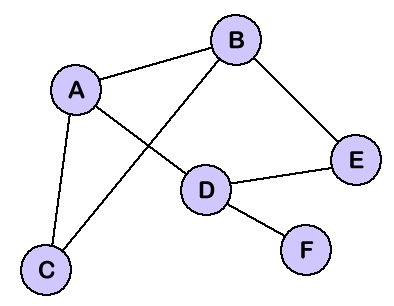
\includegraphics[height= 1.5in]{../images/Graph}}
\medskip
$\hat{y} $ assigns a class $\hat{y}[i]$ to each node (superpixel) $i$.
\bigskip
\bigskip
{\color{red}
\begin{eqnarray*}
P_\Phi(\hat{y}|x) & = & \expsoftmax_{\hat{y}}\;s_\Phi(\hat{y}|x)
\end{eqnarray*}
}

\vfill
{\color{red} $$s_\Phi(\hat{y}|x) = \sum_{i \in {\cal I}} s_i[\hat{y}[i]] + \sum_{e \in {\cal E}}\;s_e[\hat{y}[e.i],\hat{y}[e.j]]$$}

\anaslide{Exponential Softmax is Typically Unfriendly}
\bigskip
\centerline{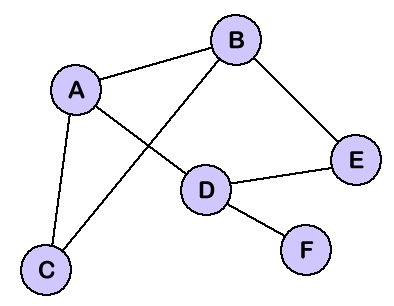
\includegraphics[height= 1.5in]{../images/Graph}}
\medskip
$\hat{y} $ assigns a class $\hat{y}[i]$ to each node (superpixel) $i$.
\bigskip
\bigskip
{\color{red}
\begin{eqnarray*}
P_\Phi(\hat{y}|x) & = & \expsoftmax_{\hat{y}}\;s_\Phi(\hat{y}|x)
\end{eqnarray*}
}

\vfill
Computing $Z$ in general is \#P hard.

\vfill
{\color{red} But special cases can be friendly and approximations can be made in unfriendly cases.}

\slide{Latent Variables}

We are often interested in models of the form

\vfill
{\color{red} $$P_\Phi(y) = \sum_z\;P_\Phi(z)P_\Phi(y|z).$$}

\vfill
Probabilistic grammar models have this form where $y$ is a sentence and $z$ is a parse tree
and $P(y|z)$ is deterministic.

\slide{A Composition of Friendlies is Typically  Unfriendly}

{\color{red} $$P_\Phi(y) = \sum_z\;P_\Phi(z)P_\Phi(y|z).$$}

\vfill
It is often the case that $P_\Phi(z)$ is friendly, and $P_\Phi(y|z)$ is friendly, but $P_\Phi(y)$ is not friendly (the sum over $z$ is intractible).

\vfill
For example $z$ might be uniformly distributed over assignments of truth values to Boolean variables (which is friendly) and $y$ might be the value of a fixed Boolean formula $\Phi$ (which is friendly given $z$).  In this case
determining if $P_\Phi(y) > 0$ is the SAT problem which is NP hard.

\slidetwo{Connectionist Temporal Classification (CTC)}
{A Successful Deep Latent Variable Model}

A speech signal
$$x = x_1,\; \ldots,\; x_{\color{red} T}$$
is labeled with a phone sequence
$$y = y_1, \ldots, y_{\color{red} N}$$
with {\color{red} $N << T$} and with $y_n \in {\cal P}$ for a set of phonemes ${\cal P}$.

\vfill
{\color{red} The length $N$ of $y$ is not determined by $x$ and the alignment between $x$ and $y$ is not given.}

\slide{CTC: A Friendly Compositions of Friendlies}

{\color{red} $$P_\Phi(y|x) = \sum_z\;P_\Phi(z|x)P_\Phi(y|z).$$}

\vfill
\begin{tabbing}
Input Signal: \hspace{3em} \=$x = x_1,\;\ldots,\;x_{\color{red} T}$ \\
Latent Label: \>$z = z_1,\;\ldots,\;z_{\color{red} T},\;\;\;z_t \in {\cal P} \cup \{\bot\}$ \\
Output: \>$y(z) = y_1,\;\ldots,\;y_{\color{red} N}\;\;\;\;\;\;{\color{red} N << T}$
\end{tabbing}

\vfill
$y(z)$ is the result of removing all the occurrences of $\bot$ from $z$:

{\color{red} $$\hspace{5em} z \hspace{7em} \Rightarrow \hspace{2em} y$$}
{\color{red} $$\bot,a_1,\bot,\bot,\bot,a_2,\bot,\bot,a_3,\bot \;\;\;\Rightarrow\;\; a_1,a_2,a_3$$}


\slide{The CTC Model}

For $z \in {\cal P} \cup \{\bot\}$ we have an embedding $e(z)$.  The embedding is a parameter of the model.

\begin{eqnarray*}
  h_1,\;\ldots,\;h_T & = & \mathrm{RNN}_\Phi(x_1,\;\ldots,\;x_T) \\
  \\
  P_\Phi(z_t|x_1,\ldots,x_T) & = & {\color{red} \softmax_{z} \;e(z)^\top h_t}
\end{eqnarray*}

\vfill
$z_1$, $\ldots$ $z_T$ are {\color{red}  all independent} given $x$ (very friendly).

\vfill
$P_\Phi(y|z)$ is {\color{red} deterministic} (very friendly).

\vfill
{\color{red} But it is not obvious whether $P_\Phi(y|x)$ is friendly.}


\slide{Dynamic Programming}
\begin{eqnarray*}
  x & = & x_1,\;\ldots,\; x_T \\
  z & = & z_1, \;\ldots,\;z_T,\;\;\;z_t \in {\cal P}\cup \{\bot\} \\
  y & = & y_1,\;\ldots,\;y_N,\;\;\;\;y_n \in {\cal P},\;\;\;N << T \\
  y(z) & = & (z_1,\;\ldots,\;z_T) - \bot
\end{eqnarray*}

\vfill

\begin{eqnarray*}
  \vec{y}_t & = & (z_1,\;\ldots,\;z_t)-\bot \\
  {\color{red} F[n,t]} & = & P(\vec{y}_{\color{red} t} = y_1,\;\ldots,\;y_{\color{red} n}) \\
  P(y) & = & F[N,T]
\end{eqnarray*}

\slide{Dynamic Programming}

\begin{eqnarray*}
  \vec{y}_t & = & (z_1,\;\ldots,\;z_t)-\bot \\
  {\color{red} F[n,t]} & = & P(\vec{y}_{\color{red} t} = y_1,\;\ldots,\;y_{\color{red} n}) \\
\end{eqnarray*}

\begin{eqnarray*}
  F[0,0] & = & 1 \\
  F[n,0] & = & 0 \;\;\;\mbox{for $n > 0$} \\
  {\color{red} F[n,t]} & = & {\color{red} P(z_t = \bot) F[n,t-1] + P(z_t = y_n)F[n-1,t-1]}
\end{eqnarray*}

\slide{Semantic Segmentation}
\centerline{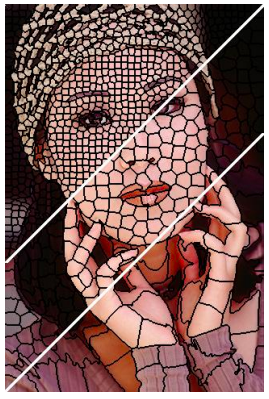
\includegraphics[height = 2.5in]{../images/SLICcolor}}
\centerline{\huge SLIC superpixels, Achanta et al.}

\vfill
We want to assign each superpixel one of $k$ semantic classes.

\vfill
For example ``person'', ``car'', ``building'', ``sky'' or ``other''.

\slide{Unfriendly Exponential Softmax}
\bigskip
\centerline{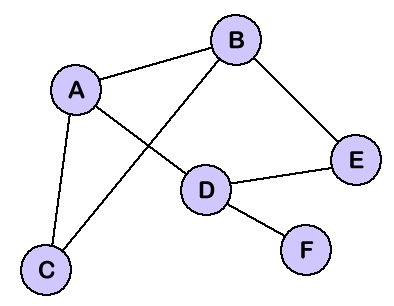
\includegraphics[height= 1.5in]{../images/Graph}}
\medskip
$\hat{y} $ assigns a class $\hat{y}[i]$ to each node (superpixel) $i$.
\bigskip
\bigskip
{\color{red}
\begin{eqnarray*}
P_\Phi(\hat{y}|x) & = & \expsoftmax_{\hat{y}}\;s_\Phi(\hat{y}|x)
\end{eqnarray*}
}

\vfill
{\color{red} $$s_\Phi(\hat{y}|x) = \sum_{i \in {\cal I}} s_i[\hat{y}[i]] + \sum_{e \in {\cal E}}\;s_e[\hat{y}[e.i],\hat{y}[e.j]]$$}

\slide{Back-Propagation Through Unfriendly Softmax}

\vfill
\begin{eqnarray*}
\mbox{intput}\; x \\
 & \vdots & \\
{\color{red} s_i[c]} & = & \ldots \\
{\color{red} s_e[c,c']} & = & \ldots \\
{\cal L} & = & - \ln\; P(y\;|\;{\color{red} s_{\cal I}[{\cal C}]},\;{\color{red} s_{\cal E}[{\cal C}, {\cal C}]})
\end{eqnarray*}

\vfill
We need to compute {\color{red} $s_i.\grad[c]$} and {\color{red} $s_e.\grad[c,c']$}.

\slide{Hyper-Graphs: More General and More Concise}

A hyper-edge is a subset of nodes.

\vfill
\centerline{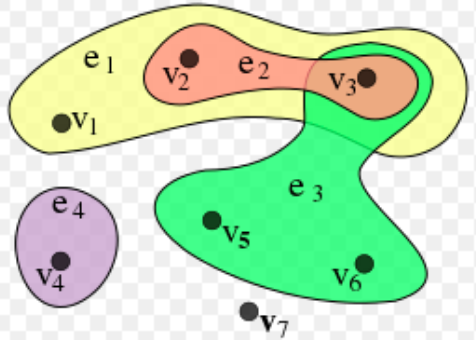
\includegraphics[height = 1.5in]{../images/HyperGraph}}


$$s(\hat{y}) = \sum_{i \in \mathrm{Nodes}}\; s_i[\hat{y}[i]]\; + \sum_{e \in \mathrm{Edges}}\;s_e[\hat{y}[e.i],\hat{y}[e.j]]$$

\vfill

$${\color{red} s(\hat{y}) = \sum_{e \in \mathrm{HyperEdges}}  \; s_e[\hat{y}[e]]}$$


\slide{Hyper-Graph Models}

We will abbreviate $s_e[\hat{y}[e]]$ as {\color{red} $s_e[\tilde{y}]$}.

\vfill
{\color{red} $\tilde{y}$ has a small number of possible values.}

\vfill
The hyper-graph model is defined by the ``tensor'' {\color{red} $s_e(\tilde{y})$}.


\slide{Backpropagation}

The input is the image $x$ and the parameter package $\Phi$

\begin{eqnarray*}
 & \vdots & \\
s_e[\tilde{y}] & = & \ldots \\
{\cal L} & = & - \ln\; P(y\;|\;s_{\cal E}[{\cal Y}])
\end{eqnarray*}

\vfill We abbreviate $P(\hat{y}\;|\;s_{\cal E}[{\cal Y}])$ as {\color{red} $P_s(\hat{y})$} --- the distribution on $\hat{y}$ defined by the tensor $s$.
\vfill
We need to compute {\color{red} $\nabla_s -\ln P_s(y)$}, or equivalently, {\color{red} $s_e.\grad[\hat{y}[e]]$}.

\slide{Back-Propagation Through An Exponential Softmax}

\begin{eqnarray*}
  {\cal L}(s,y) & = & - \ln \left(\frac{1}{Z(s)}\;e^{s(y)}\right) \\
  \\
  & = & \ln Z(s) - s(y) \\
  \\
  \\
  s_e.\mathrm{grad}[\tilde{y}]
    & = & \left(\frac{1}{Z} \sum_{\hat{y}} e^{s(\hat{y})} \left(\partial s(\hat{y})/\partial s_e[\tilde{y}]\right)\right)
    - \left(\partial s(y) /\partial s_e[\tilde{y}]\right)
\end{eqnarray*}

\slide{Back-Propagation Through An Exponential Softmax}

\bigskip
\begin{eqnarray*}
    s_e.\mathrm{grad}[\tilde{y}]
    & = & \left(\frac{1}{Z} \sum_{\hat{y}} e^{s(\hat{y})} \left(\partial s(\hat{y})/\partial s_e[\tilde{y}]\right)\right)
    - \left(\partial s(y) /\partial s_e[\tilde{y}]\right)    \\
    \\
    & = & \left(\sum_{\hat{y}} P_s(\hat{y}) \left(\partial s(\hat{y})/\partial s_e[\tilde{y}]\right)\right)
    - \left(\partial s(y) /\partial s_e[\tilde{y}]\right)    \\
    \\
    & = & E_{\hat{y} \sim P_s}\bbone[\hat{y}[e] = \tilde{y}]
    - \mathbbm{1}[y[e] = \tilde{y}] \\
    \\
    & = & {\color{red} P_{\hat{y} \sim P_s}(\hat{y}[e] = \tilde{y})}
      - \mathbbm{1}[y[e] = \tilde{y}]
\end{eqnarray*}

\slide{Hyperedge Marginals}

\begin{eqnarray*}
    s.\mathrm{grad}[e,\tilde{y}]
    & = &  {\color{red} P_{\hat{y} \sim P_s}(\hat{y}[e] = \tilde{y})} - \bbone[y[e] = \tilde{y}] \\
\end{eqnarray*}

\vfill
We write {\color{red} $P_e(\tilde{y})$} for the {\color{red} hyperedge marginal} $P_{\hat{y} \sim P_s}(\hat{y}(e) = \tilde{y})$.

\vfill
To back-propagate log loss on a labeling of an unfriendly MRF {\color{red} it suffices to compute (or perhaps approximate)
the current model's hyperedge marginals ${\color{red} P_e(\tilde{y})}$.}

\slide{Tree-Structured Models are Friendly}

\centerline{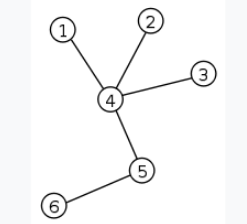
\includegraphics[height= 2in]{../images/Tree}}

\vfill
Tree structure models can always be locally renormalized to form ``autoregressive'' models that
predict one node at a time.

\vfill
Also, the hyperedge marginals can be computed exactly.


\anaslide{Belief Propagation}

\centerline{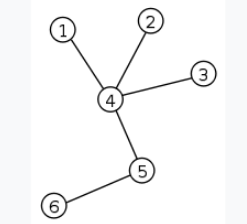
\includegraphics[height=1.5in]{../images/Tree}}

\vfill
Belief Propagation is a message passing procedure (actually dynamic programming).

\vfill
For each edge $\{i,j\}$ and possible value $\tilde{y}$ for node $i$ we define {\color{red} $Z_{j \rightarrow i}[\tilde{y}]$}
to be  the partition function for the subtree attached to $i$ through $j$ and
with $\hat{y}[i]$ restricted to $\tilde{y}$.

\vfill
The function $Z_{j \rightarrow i}$ on the possible values of node $i$ is called the {\bf message} from $j$ to $i$.

\vfill
The reverse direction message $Z_{i \rightarrow j}$ is defined similarly.

\slide{Computing the Messages}

\centerline{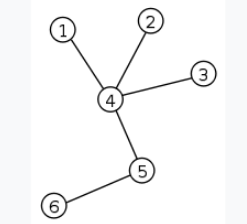
\includegraphics[height=2.0in]{../images/Tree}}

\vfill
\begin{eqnarray*}
  Z_{j\rightarrow i}[\tilde{y}] & = & \sum_{\tilde{y}'}  e^{s_j[\tilde{y}'] + s[\{j,i\},\{\tilde{y}',\tilde{y}\}]}
    \left(\prod_{k \in N(j),\;k \not = i}\;Z_{k\rightarrow j}[\tilde{y}']\right)
\end{eqnarray*}

\anaslide{Computing Node Marginals from Messages}

\centerline{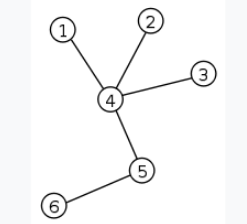
\includegraphics[height=1.5in]{../images/Tree}}

\begin{eqnarray*}
Z_i(\tilde{y}) & \doteq & \sum_{\hat{y}:\; \hat{y}[i] = \tilde{y}} \;e^{s(\hat{y})} \\
\\
& = & e^{s_i[\tilde{y}]} \left(\prod_{j\in N(i)} Z_{j \rightarrow i}[\tilde{y}]\right) \\
\\
{\color{red} P_i(\tilde{y})} & = & Z_i(\tilde{y})/Z,\;\;\;\;\; Z = \sum_{\tilde{y}}\;Z_i(\tilde{y})
\end{eqnarray*}


\anaslide{Computing Edge Marginals from Messages}

\begin{eqnarray*}
Z_{\{i,j\}}(\tilde{y}) & \doteq & \sum_{\hat{y}:\; \hat{y}[\{i,j\}] = \tilde{y}} \;e^{s(\hat{y})} \\
\\
& = & e^{s[i,\tilde{y}[i]] + s[j,\tilde{y}[j]] +s[\{i,j\},\tilde{y}]} \\
& & \prod_{k\in N(i),\;k \not = j} Z_{k \rightarrow i}[\tilde{y}[i]] \\
& & \prod_{k\in N(j),\;k \not = i} Z_{k \rightarrow j}[\tilde{y}[j]] \\
\\
{\color{red} P_{\{i,j\}}(\tilde{y})} & = & Z_{\{i,j\}}(\tilde{y})/Z
\end{eqnarray*}

\slide{Loopy BP}

Message passing is also called belief propagation (BP).

\vfill
In a graph with cycles it is common to do {\bf Loopy BP}.

\vfill
This is done by initializing all message $Z_{i \rightarrow j}[\tilde{y}] = 1$ and then repeating (until convergence) the updates
\vfill
\begin{eqnarray*}
  \tilde{Z}_{j \rightarrow i}[\tilde{y}] & = & \frac{1}{Z_{j \rightarrow i}}\;Z_{j \rightarrow i}[\tilde{y}] \;\;\;\;\;Z_{j \rightarrow i} = \sum_{\tilde{y}} Z_{j \rightarrow i}[\tilde{y}] \\
  \\
  \\
  Z_{j\rightarrow i}[\tilde{y}] & = & \sum_{\tilde{y}'}  e^{s[j,\tilde{y}'] + s[\{j,i\},\{\tilde{y}',\tilde{y}\}]}
    \left(\prod_{k \in N(j),\;k \not = i}\;\tilde{Z}_{k\rightarrow j}[\tilde{y}']\right)
\end{eqnarray*}

\slide{Other Methods of Approximating Hyperedge Marginals}

MCMC Sampling

\vfill
Constrastive Divergence

\vfill
Pseudo-Liklihood


\slide{Sampling}
The quantities ${\color{red} P_e(\tilde{y})}$ are {\bf hyperedge marginals}.

\vfill
We can estimate the hyperedge marginals by sampling $\hat{y}$ from $P_s(\hat{y})$.

\slide{Monte Carlo Markov Chain (MCMC) Sampling}

\centerline{\bf Metropolis Algorithm}

\vfill
Pick an initial graph label $\hat{y}$ and then repeat:

\begin{enumerate}
\item Pick a ``neighbor'' $\hat{y}'$ of $\hat{y}$ uniformly at random.  The neighbor relation must be symmetric.  Perhaps Hamming distance one.

  \vfill
\item If $s(\hat{y}') > s(\hat{y})$ update $\hat{y} = \hat{y}'$

  \vfill
\item If $s(\hat{y}') \leq s(\hat{y})$ then update $\hat{y} = \hat{y}'$ with probability $e^{-(s(\hat{y}) - s(\hat{y}'))}$
  \end{enumerate}  

\slide{Markov Processes and Stationary Distributions}

A Markov process is a process defined by a fixed state transition probability $P(\hat{y}'|\hat{y}) = M_{\hat{y}',\hat{y}}$.

\vfill
Let $P^t$ the probability distribution for time $t$.

\vfill
$$P^{t+1} = MP^t$$

\vfill
If every state can be reached form every state (ergodic process) then $P^t$ converges to a unique {\bf stationary distribution} $P^\infty$

\vfill
$$P^\infty = MP^\infty$$

\slide{Metropolis Theorem}

To verify that the Metropolis process has the correct stationary distribution we simply verify that $MP = P$ where $P$
is the desired distribution.

\vfill
This can be done by checking that under the desired distribution the flow from $\hat{y}$ to $\hat{y}'$
equals the flow from $\hat{y}'$ to $\hat{y}$ ({\bf detailed balance}).

\slide{Metropolis Theorem}

For $s(\hat{y}) \geq s(\hat{y}')$

\vfill
\begin{eqnarray*}
  \mathrm{flow}(\hat{y}' \rightarrow \hat{y}) &  = & \frac{1}{Z}e^{s(\hat{y}')} \frac{1}{N} \\
  \\
\mathrm{flow}(\hat{y} \rightarrow \hat{y}') & = & \frac{1}{Z}e^{s(\hat{y})} \frac{1}{N} e^{-\Delta s} = \frac{1}{Z} e^{s(\hat{y}')} \frac{1}{N}
\end{eqnarray*}

\vfill
But detailed balance is not required in general (see Hamiltonian MCMC).

\slide{Gibbs Sampling}

The Metropolis algorithm wastes time by rejecting proposed moves.

\vfill
Gibbs sampling avoids this move rejection.

\vfill
In Gibbs sampling we select a node $i$ at random and change that node by drawing a new node value conditioned on the current values of the other nodes.

\slide{Gibbs Sampling}

Markov Blanket Property:
$$P_s(\hat{y}[i] \;|\;\hat{y} \backslash i) = P_s(\hat{y}[i] \;|\; \hat{y}[N(i)])$$
  
\vfill
Gibbs Sampling, Repeat:

\begin{itemize}
\item   Select $i$ at random

\item draw $\tilde{y}$ from $P_s(\hat{y}[i] \;|\;\hat{y} \backslash i)$

\item $\hat{y}[i] = \tilde{y}$
\end{itemize}

\slide{Gibbs Sampling Theorem}

$P_s(\hat{y})$ is a stationary distribution of Gibbs Sampling.

\vfill
\begin{itemize}
\item   Select $i$ at random

\item draw $\tilde{y}$ from $P_s(\hat{y}[i] \;|\;\hat{y} \backslash i)$

\item $\hat{y}[i] = \tilde{y}$
\end{itemize}


\vfill
The distribution before the update equals the distribution after the update.

\slide{Pseudolikelihood}

In pseudolikelihood we replace the objective $- \ln P_s(\hat{y})$ with the objective $- \ln \tilde{Q}_s(\hat{y})$ where

\vfill
\begin{eqnarray*}
  \tilde{Q}_s(y) & \doteq & \prod_i \;P_s(y[i] \;|\;y\backslash i) \\
  \\
  {\cal L}(s) & \doteq & - \ln \tilde{Q}_s(y) \\
  \\
  {\color{red} s.\mathrm{grad}[e,\tilde{y}]} & = & {\color{red} \sum_i \frac{- \partial \ln P_s(y[i] \;|\;y\backslash i)}{\partial s[e,\tilde{y}]}
  \hspace{3em} \mbox{immediate gradient!}}
\end{eqnarray*}


\slide{Pseudolikelihood Theorem}

$$\argmin_Q \; E_{y \sim \mathrm{Pop}} \;-\ln \tilde{Q}(y) = \mathrm{Pop}$$

\vfill

\slide{Proof I}

{\color{red} $$E_{y \sim \mathrm{Pop}}\;\ln \widetilde{\mathrm{Pop}}(y) = E_{y \sim \mathrm{Pop}}\;\ln \mathrm{Pop}(y)$$}
{\huge
\begin{eqnarray*}
\mbox{Proof:}\hspace{5em}\pop(y) & = & \prod_i P(y[i]\;|\; y[<\;i]) \\
\ln \pop(y) & = & \sum_i \; \ln P(y[i]\;|\; y[<\;i]) \\
E_{y \sim \pop}\;\ln \pop(y) & = & \sum_i \;E_{y \sim \pop} \; \ln P(y[i]\;|\; y[<\;i]) \\
& = & \sum_i \;E_{y \sim \pop} \;\ln P(y[i]\;|\; y\backslash i) \\
& = & E_{y\sim \pop}\;\widetilde{\pop}(y)
\end{eqnarray*}
}

\slide{Proof II}
$$\min_{Q} \;E_{y \sim \mathrm{Pop}}\;-\ln \tilde{Q}(y) \;\;\leq \;\; E_{y \sim \mathrm{Pop}}\;-\ln \widetilde{\mathrm{Pop}}(y)$$

\vfill
If we can show

$$\min_{Q} \;E_{y \sim \mathrm{Pop}}\;-\ln \tilde{Q}(y) \;\;\geq \;\; E_{y \sim \mathrm{Pop}}\;-\ln \widetilde{\mathrm{Pop}}(y)$$

Then the minimizer (the argmin) is $\mathrm{Pop}$ as desired.

\slide{Proof III}

We will prove the case of two nodes.

\vfill
\begin{eqnarray*}
  & & \min_Q \;E_{y\sim \mathrm{Pop}}{-\ln Q(y[1]|y[2])\;Q(y[2]|y[1])} \\
  \\
  & \geq & \min_{P_1,P_2} E_{y \sim \mathrm{Pop}}{-\ln P_1(y[1]|y[2])\;P_2(y[2]|y[1])} \\
  \\
  & = & \min_{P_1} E_{y \sim \mathrm{Pop}}{-\ln P_1(y[1]|y[2])} + \min_{P_2} E_{y \sim \mathrm{Pop}}{-\ln P_2(y[2]|y[1])} \\
  \\
  & = & E_{y \sim \mathrm{Pop}}{-\ln \mathrm{Pop}(y[1]|y[2])} + E_{y \sim \mathrm{Pop}}{-\ln \mathrm{Pop}(y[2]|y[1])} \\
  \\
  & = & E_{y \sim \mathrm{Pop}}{-\ln \widetilde{\mathrm{Pop}}(y|x)}
\end{eqnarray*}

  
\slideplain{Contrastive Divergence}
{\bf Algorithm (CDk)}: Run $k$ steps of MCMC for $P_s(\hat{y})$ {\bf starting from $y$} to get $\hat{y}$.

\vfill
Then set
$$s.\mathrm{grad}[e,\tilde{y}] = \mathbbm{1}[\hat{y}[e] = \tilde{y}] - \mathbbm{1}[y[e]= \tilde{y}]$$

\vfill
    {\bf CD Theorem}: If $P_s(\hat{y}) = \mathrm{Pop}$ then
    
    $$E_{y \sim \mathrm{Pop}}\; \mathbbm{1}[\hat{y}[e] = \tilde{y}] - \mathbbm{1}[y[e]= \tilde{y}] = 0$$

\vfill
{\bf Here we can take $k=1$ --- \bf no mixing time required}.

\slide{Summary}

We are often interested in probability distributions on structured objects such as sentence or images.

\vfill
Graphical models define softmax distributions on structured values.

\vfill
It is infeasible to enumerate all sentences or all images.

\vfill
However, some graphical models sometimes yield friendly distributions and methods exist
for training unfriendly graphical models.
\slide{END}

}
\end{document}
